\documentclass[12pt]{article}
\usepackage[margin=1 in]{geometry}
\usepackage{graphicx}
\usepackage[utf8]{inputenc}
\usepackage{listings}
\usepackage{graphicx}


\title{\vspace{-4em}Stat 628 Module 2: BodyFat}
\author{YUKUN FANG \quad MENGKUN CHEN \quad JIAYI SHEN}
\date{}

\begin{document}
\sffamily

\maketitle
\section{\sffamily Introduction(YF)}
A variety of popular health books suggest that the readers assess their 
health, at least in part, by estimating their percentage of body fat.
The goal of the project is to come up with 
a simple and accurate way of deteriming body fat percentage of males
based on readily available clinical measurements and find the rule of thumb.\\
\textbf{Our rule of thumb:} $$ {\rm BodyFat} =  = -29.7950 + 0.14W + 0.04C + 0.05A+ 0.03H +0.02T + 0.17{\rm AGE}$$
\textbf{W} stands for weight, \textbf{C} stands for chest, \textbf{A} stands for abdomen, \textbf{H} stands for hip, \textbf{T} for thigh.
\section{\sffamily Background(YF)}
The data set contains measurements from 252 men who had their body fat 
percentage accurately measured via underwater weighing. Notice that the 
outcome variable is body fat percentage and he set of predictors are 
every variable except ID number, body fat percentage, and density.
\section{\sffamily Motivation and Statement(YF)}
\subsection{\sffamily Motivation}
In the beginning we have used linear model step selection by using 
AIC or BIC to find the best model which may lead to multicollinearity during fitting the model.
So we use the principal component analysis to find the PC(principal components), and
then use PCs to find linear model.

\subsection{\sffamily Statement of the Model}
\textbf{First}, we calculate the covariance matrix of the data set for 15 variables without the three.
Then we calculate the eigenvalues and the eigenvectors of the matrix.
Then calculate the cumsum of the eigenvalues and divided by sum of eigenvectors and equals to cumvariance. 
This value is the main result which is use to find the principle components.\\
\textbf{Second}, we plot the cumvariance and select the top two eigenvalues as the PCs: PC1 and PC2.
Then we need to remove the variables whose coefficients are so small with big p-value for t-statistics.\\
\textbf{At last}, we use PCs as variables to fit the linear model to diagnose and remedy it.

\section{\sffamily Estimation and Inference of Parameters(YF)}
After the calculation, we get the 2 PCs:
$$PC_1 = 0.88W + 0.24 C + 0.30
A + 0.20  H + 0.14 T$$
$$PC_2 = 0.96{\rm AGE} $$
Then fit the model and get a not good model. 
After we diagnose and remedy it, we change PCs by the primary variables and get the final model.
\section{\sffamily Model Diagnostics(YF)}
We draw these two plots and find there exists one outlier NO.39.
\begin{figure}[ht]
	\centering
	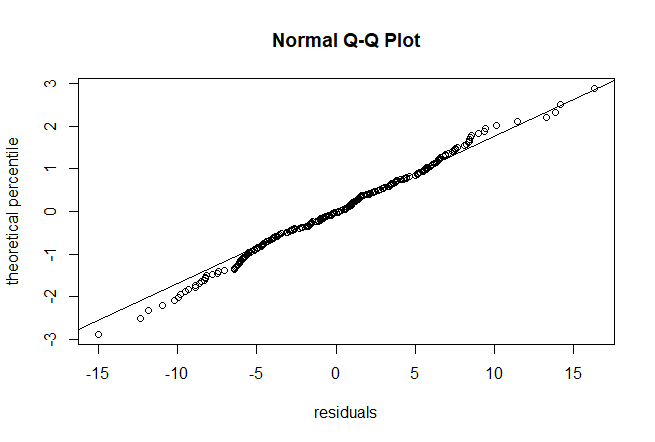
\includegraphics[width=6cm,height=4cm]{2.png}
	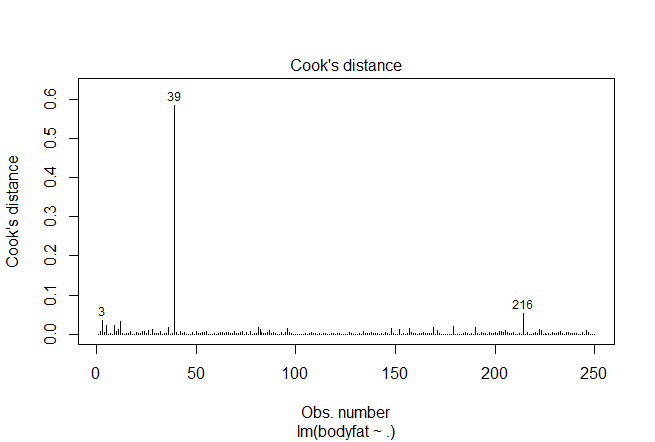
\includegraphics[width=6cm,height=4cm]{3.png}  
\end{figure}
After removing that, we refit the model and get the result:
And the summary shows that is fits well.
$${\rm BODYFAT} = -29.7950 + 0.1644PC_1 + 0.1759PC_2$$
We can get r-square=$50\%$ and residual table
\begin{table}[ht]
    \centering
    \begin{tabular}{rrrrr}
      \hline
     & Estimate & Std. Error & t value & Pr($>$$|$t$|$) \\ 
      \hline
    (Intercept) & -27.5858 & 3.0069 & -9.17 & $<2e-16$ \\ 
      pc1 & 0.1644 & 0.0115 & 14.25 & $<2e-16$  \\ 
      pc2 & 0.1759 & 0.0282 & 6.25 & $1.83e-09$ \\ 
       \hline
    \end{tabular}
    \end{table}
The final model: $${\rm BODYFAT} = -29.7950 + 0.14W + 0.04C + 0.05A+ 0.03H +0.02T + 0.17{\rm AGE}$$
\section{\sffamily Strengths and Weakness(YF)}
\begin{itemize}
    \item \textbf{Strengths}: This method is wild range of use for any other problem and robust for multicollinearity. Also it is easy to understand and 
    get the result.
    \item \textbf{Weakness}: If someone has some body statistics out of
    range, it may casue bad result. Also the R-square is not close to 1 which means 
    we need to improve the model.
\end{itemize}
\section{\sffamily Conclusion}
    \centerline{Summary: Yukun Fang~~~~~~~Code: Mengkun Chen~~~~~~~~~~~Slides: Jiayi Shen}
\end{document}